\section{NODE SOFTWARE}

\subsection{Description of the implementation}

The system extends the functionality of the Mbed-OS \acrshort{lorawan} example provided by the teachers, in which an event-queue is provided.

ThIS event-queue provides an asynchronous event dispatcher, in this case for \acrshort{lorawan} events. And, for any event that happens in the system, a callback will be done to process that situation. This working can be seen in the next figure.

\begin{figure}[H]
    \centering
    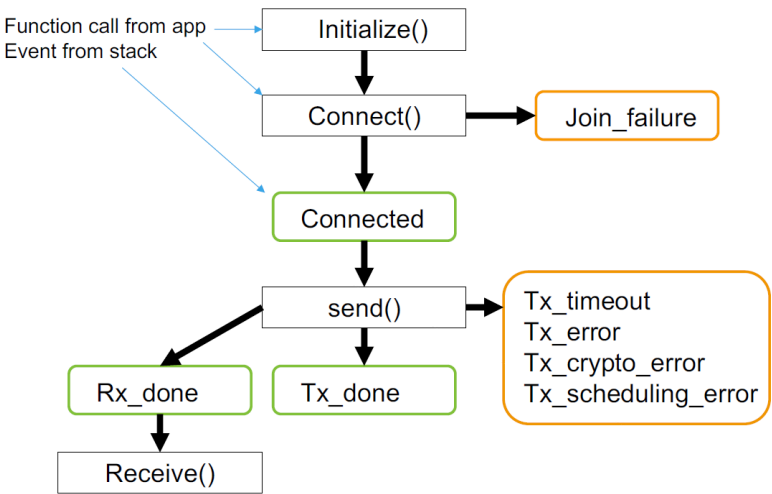
\includegraphics[width=0.7\textwidth]{images/4/event-queue.png}
    \caption{EventQueue solution REFERENCIA DE LAS DIAPOS O A LOS PROFES O CAMBIARLO}
    \label{fig:events}
\end{figure}

The solution is implemented by extending the previous event-queue. This event queue will detect possible TX windows in the \acrshort{lorawan} PHY layer and create an event to send a new message with data regarding the measurements of the plant sensors. These sensors are: 
GPS, brightness, soil moisture, humidity, temperature, linear acceleration, RGB data and led status.

To obtain this data, measurement threads are changed from the previous project, these threads read new values each 5 seconds and store the data in an mutex-controlled structure to send the data later.

The threads are:
\begin{itemize}
    \item Main thread with the event-queue.
    \item I2C thread.
    \item GPS thread.
\end{itemize}
\clearpage
\subsection{Threads and communication design} % Comentar los cambios realizados
\clearpage
\subsection{Frame design}